\documentclass[aspectratio=169, table, 12pt]{beamer}

\usepackage{colortbl}
\usepackage{xcolor}
\usepackage{listings}
\usepackage{tabularx}
\usepackage{tikz}
\usetikzlibrary{arrows.meta, positioning, calc, fit, shapes.geometric}

\makeatletter
\def\input@path{{../theme/}}
\makeatother
\graphicspath{{../theme/}{../../figures/}}
\usetheme{Pradita}

\definecolor{praditagreen}{RGB}{37, 113, 71}

% Tema membuat garis tabel berwarna putih. Dikembalikan agar tabel terbaca.
\arrayrulecolor{black}
\setlength{\arrayrulewidth}{0.5pt}

% Menempatkan gambar di tengah kolom, mendatar sekaligus tegak. Lebarnya
% dipenuhi selebar kolom. Bila hasilnya melebihi tinggi yang disediakan,
% tingginya yang menjadi pembatas, sehingga gambar tidak menembus bingkai.
\newsavebox{\kotakkolom}
\newcommand{\gambarkolom}[2][0.72\textheight]{%
  \sbox{\kotakkolom}{\resizebox{\linewidth}{!}{#2}}%
  \begin{minipage}[c][#1][c]{\linewidth}%
    \centering
    \ifdim\dimexpr\ht\kotakkolom+\dp\kotakkolom\relax>#1\relax
      \resizebox{!}{#1}{#2}%
    \else
      \usebox{\kotakkolom}%
    \fi
  \end{minipage}%
}

\lstdefinestyle{PythonStyle}{
  language=Python,
  basicstyle=\ttfamily\scriptsize,
  keywordstyle=\color{blue}\bfseries,
  commentstyle=\color{gray}\itshape,
  stringstyle=\color{red},
  breaklines=true,
  frame=lines,
  backgroundcolor=\color{lightgray!10},
  tabsize=2,
  showstringspaces=false
}

\lstdefinelanguage{bash}{
  keywords={},
  basicstyle=\ttfamily\scriptsize,
  ndkeywords={cd, python, bash, source},
  ndkeywordstyle=\color{purple}\bfseries,
  sensitive=true,
  commentstyle=\color{gray},
  breaklines=true,
  frame=lines,
  backgroundcolor=\color{lightgray!10},
  tabsize=2,
  comment=[l]{\#},
  showstringspaces=false
}

\title{\Huge{Orchestration-Driven SOA}}
\subtitle{IF231303 Arsitektur Perangkat Lunak}
\author{Alfa Yohannis}

\begin{document}

\frame{\titlepage}

\begin{frame}{{\Large Tujuan Pembelajaran}}
  \vspace{10pt}
  \begin{enumerate}
    \item Menjelaskan taksonomi empat lapisan layanan beserta tugas mesin
          orkestrasi yang merangkainya.
    \item Membedakan alur kerja yang tertulis pada satu tempat dari alur kerja
          yang tersebar di dalam layanan.
    \item Mengukur tambahan lompatan, biaya menyisipkan satu langkah, dan
          jumlah alur kerja yang terdampak ketika satu layanan berubah.
  \end{enumerate}

  \vspace{10pt}
  {\small Contoh bab ini adalah pemesanan valuta asing enam langkah, dijalankan
  dengan dua cara yang hasilnya sama persis.}
\end{frame}

\begin{frame}{{\Large Pendahuluan}}
  \vspace{8pt}
  \begin{itemize}\small
    \item Layanan ditata berlapis, lalu dirangkai satu mesin orkestrasi yang
          memegang seluruh urutan langkah.
    \item OASIS menyusun model acuannya, sedangkan urutan langkahnya ditulis
          dalam bahasa tersendiri seperti WS-BPEL.
    \item Hohpe dan Woolf menyebut komponen semacam itu \textit{process
          manager}, yaitu pemegang urutan sekaligus keadaan proses.
  \end{itemize}

  \vspace{8pt}
  {\small Dua hal membedakannya dari Bab 11 dan Bab 13, yaitu pemakaian ulang
  yang didorong sejauh mungkin, dan alur kerja yang seluruhnya tertulis di
  dalam mesin.}
\end{frame}

\begin{frame}{{\Large Empat Lapisan Layanan}}
  \vspace{6pt}
  \centering
  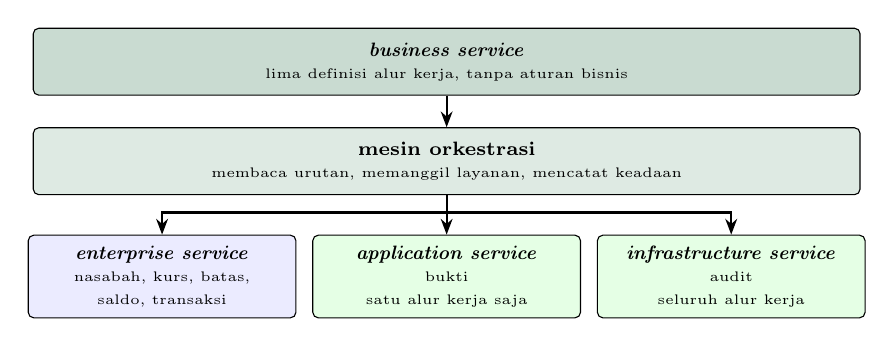
\begin{tikzpicture}[
    lapis/.style={draw, rounded corners=2pt, minimum width=10.5cm,
      minimum height=0.85cm, align=center, font=\scriptsize\bfseries},
    kecil/.style={draw, rounded corners=2pt, minimum width=3.4cm,
      minimum height=1.05cm, align=center, font=\scriptsize\bfseries},
    panah/.style={-{Stealth[length=2mm]}, thick}
  ]
    \node[lapis, fill=praditagreen!25] (bisnis) {\textit{business service}\\
      {\tiny\mdseries lima definisi alur kerja, tanpa aturan bisnis}};
    \node[lapis, fill=praditagreen!15, below=0.4cm of bisnis] (mesin)
      {mesin orkestrasi\\
      {\tiny\mdseries membaca urutan, memanggil layanan, mencatat keadaan}};
    \node[kecil, fill=green!10, below=0.5cm of mesin] (app)
      {\textit{application service}\\
      {\tiny\mdseries bukti}\\
      {\tiny\mdseries satu alur kerja saja}};
    \node[kecil, fill=blue!8, left=0.2cm of app] (ent)
      {\textit{enterprise service}\\
      {\tiny\mdseries nasabah, kurs, batas,}\\
      {\tiny\mdseries saldo, transaksi}};
    \node[kecil, fill=green!10, right=0.2cm of app] (inf)
      {\textit{infrastructure service}\\
      {\tiny\mdseries audit}\\
      {\tiny\mdseries seluruh alur kerja}};
    \draw[panah] (bisnis) -- (mesin);
    \draw[panah] (mesin.south) -- ++(0,-0.22) -| (ent.north);
    \draw[panah] (mesin.south) -- ++(0,-0.22) -| (app.north);
    \draw[panah] (mesin.south) -- ++(0,-0.22) -| (inf.north);
  \end{tikzpicture}

  \vspace{6pt}
  {\small Seluruh panah berangkat dari mesin orkestrasi. Tidak ada satu pun
  panah antar layanan.}
\end{frame}

\begin{frame}{{\Large Ketujuh Layanan dan Pemakainya}}
  \vspace{6pt}
  \centering
  \small
  \begin{tabularx}{0.95\textwidth}{|l|l|l|X|}
    \hline
    \textbf{Layanan} & \textbf{Lapisan} & \textbf{Dipakai} & \textbf{Kemampuannya} \\
    \hline
    \texttt{nasabah} & \textit{enterprise} & 4 dari 5 & Memastikan nasabah terdaftar dan aktif \\
    \hline
    \texttt{kurs} & \textit{enterprise} & 3 dari 5 & Menghitung kurs jual dan nilai rupiah \\
    \hline
    \texttt{batas} & \textit{enterprise} & 2 dari 5 & Menolak pesanan yang melewati pagu \\
    \hline
    \texttt{saldo} & \textit{enterprise} & 3 dari 5 & Memotong saldo rupiah nasabah \\
    \hline
    \texttt{transaksi} & \textit{enterprise} & 4 dari 5 & Menulis satu baris ke buku transaksi \\
    \hline
    \texttt{bukti} & \textit{application} & 1 dari 5 & Menyusun teks bukti pemesanan \\
    \hline
    \texttt{audit} & \textit{infrastructure} & 5 dari 5 & Menyimpan jejak alur kerja selesai \\
    \hline
  \end{tabularx}
\end{frame}

\begin{frame}[fragile]{{\Large Versi Orkestrasi: Komponen dan Kode}}
  \vspace{2pt}
  \begin{columns}[c]
    \begin{column}{0.5\textwidth}
      \gambarkolom[0.62\textheight]{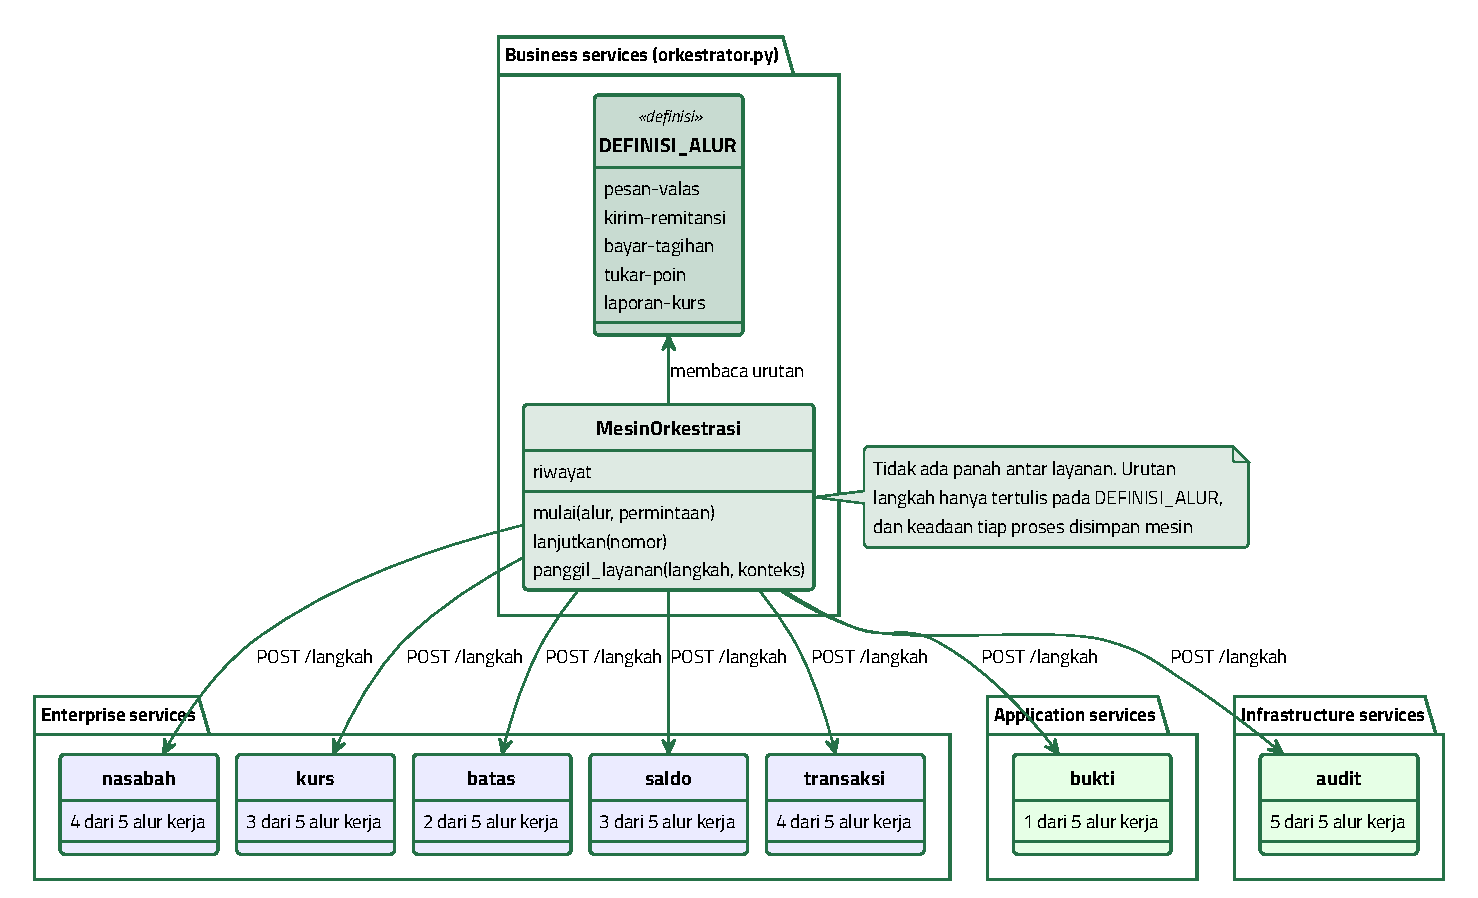
\includegraphics{kelas-odsoa.pdf}}
    \end{column}
    \begin{column}{0.48\textwidth}
\begin{lstlisting}[style=PythonStyle]
DEFINISI_ALUR = {
  "pesan-valas": ["nasabah", "kurs",
    "saldo", "transaksi", "bukti",
    "audit"],
  "tukar-poin": ["nasabah",
    "transaksi", "audit"],
  "laporan-kurs": ["kurs", "audit"],
}
\end{lstlisting}
      {\scriptsize Urutan langkah hanya tertulis di satu berkas. Layanan tidak
      mengenal tetangganya sama sekali.}
    \end{column}
  \end{columns}
\end{frame}

\begin{frame}{{\Large Versi Orkestrasi: Urutan Panggilan}}
  \vspace{2pt}
  \begin{columns}[c]
    \begin{column}{0.47\textwidth}
      \gambarkolom[0.74\textheight]{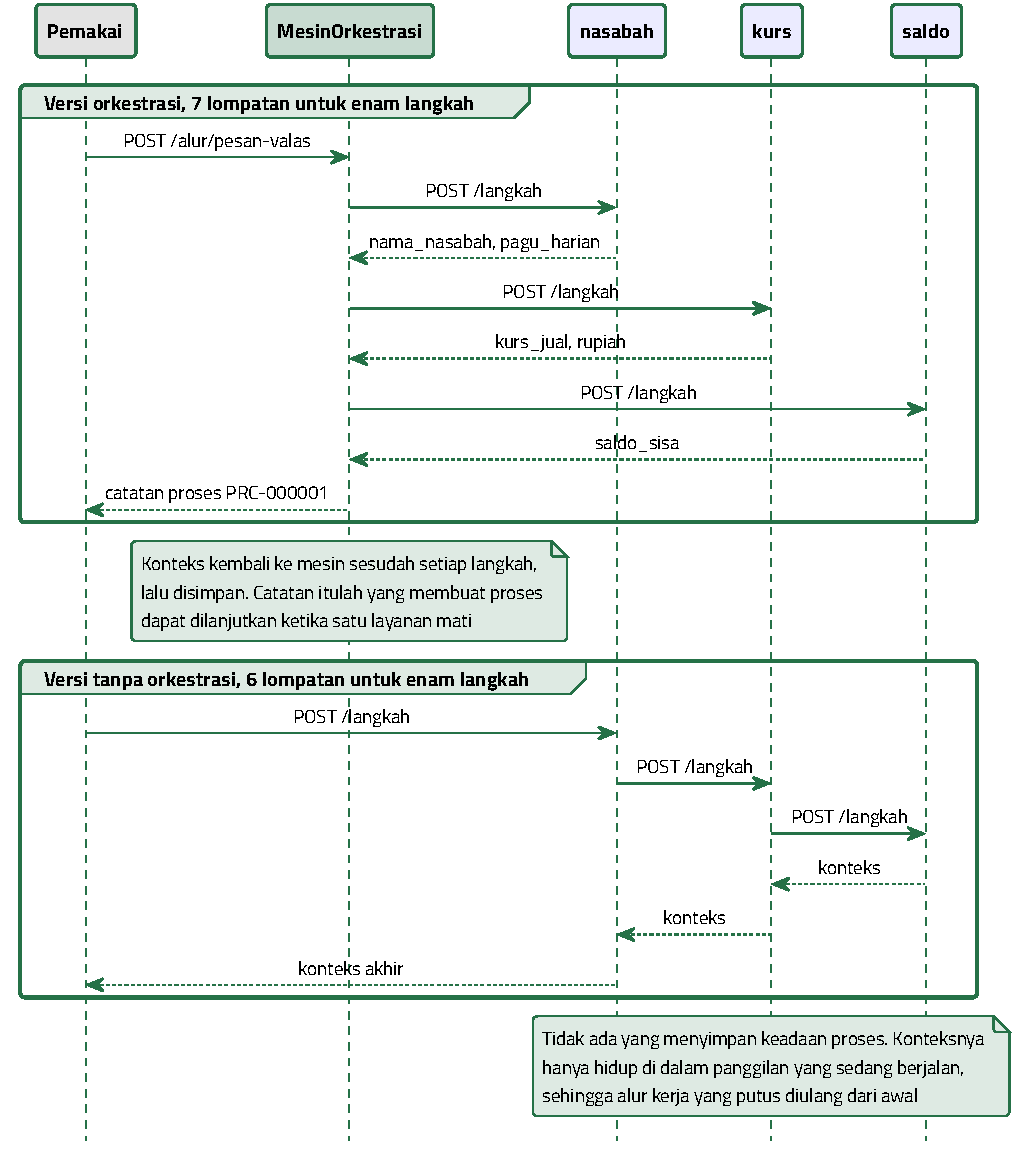
\includegraphics{sekuens-odsoa.pdf}}
    \end{column}
    \begin{column}{0.51\textwidth}
      \begin{itemize}\small
        \item Konteks kembali ke mesin sesudah setiap langkah, lalu disimpan.
        \item Alur kerja enam langkah menempuh tujuh lompatan, yaitu satu
              menuju mesin ditambah enam menuju layanan.
        \item Catatan keadaan itulah yang membuat proses dapat dilanjutkan
              ketika satu layanan mati.
        \item Nomor prosesnya dikembalikan kepada pemanggil, misalnya
              \texttt{PRC-000001}.
      \end{itemize}
    \end{column}
  \end{columns}
\end{frame}

\begin{frame}[fragile]{{\Large Versi Tanpa Orkestrasi: Kode Penerus}}
  \vspace{4pt}
\begin{lstlisting}[style=PythonStyle]
# berantai/kurs.py, potongan alur kerja yang dipegang layanan ini.
BERIKUTNYA = "saldo"

def buat_aplikasi():
  """Membentuk aplikasi Flask layanan kurs beserta penerusnya."""
  return pembantu.buat_layanan("kurs", BERIKUTNYA)
\end{lstlisting}
  \vspace{4pt}
  \begin{itemize}\small
    \item Setiap layanan memegang satu potong urutan, yaitu nama penerusnya
          sendiri.
    \item Tidak ada satu berkas pun yang memuat alur kerjanya secara utuh,
          sebab urutannya tersebar di enam berkas.
    \item Enam langkah menempuh enam lompatan, sebab konteksnya tidak pernah
          kembali ke belakang.
  \end{itemize}
\end{frame}

\begin{frame}{{\Large Versi Tanpa Orkestrasi: Urutan Panggilan}}
  \vspace{8pt}
  \centering
  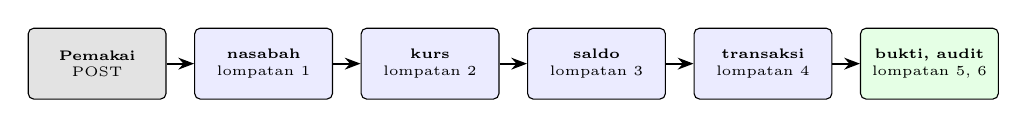
\begin{tikzpicture}[
    tahap/.style={draw, rounded corners=2pt, minimum width=1.75cm,
      minimum height=0.9cm, align=center, font=\tiny\bfseries},
    panah/.style={-{Stealth[length=2mm]}, thick}
  ]
    \node[tahap, fill=gray!22] (u) {Pemakai\\
      {\tiny\mdseries POST}};
    \node[tahap, fill=blue!8, right=0.35cm of u] (n) {nasabah\\
      {\tiny\mdseries lompatan 1}};
    \node[tahap, fill=blue!8, right=0.35cm of n] (k) {kurs\\
      {\tiny\mdseries lompatan 2}};
    \node[tahap, fill=blue!8, right=0.35cm of k] (s) {saldo\\
      {\tiny\mdseries lompatan 3}};
    \node[tahap, fill=blue!8, right=0.35cm of s] (t) {transaksi\\
      {\tiny\mdseries lompatan 4}};
    \node[tahap, fill=green!10, right=0.35cm of t] (b) {bukti, audit\\
      {\tiny\mdseries lompatan 5, 6}};
    \draw[panah] (u) -- (n);
    \draw[panah] (n) -- (k);
    \draw[panah] (k) -- (s);
    \draw[panah] (s) -- (t);
    \draw[panah] (t) -- (b);
  \end{tikzpicture}

  \vspace{8pt}
  \begin{itemize}\small
    \item Konteksnya hanya hidup di dalam panggilan yang sedang berjalan.
    \item Tidak ada tempat menyimpan keadaan, sehingga alur kerja yang putus
          wajib diulang dari langkah pertama.
    \item Menyisipkan langkah baru berarti menyunting layanan yang sedang
          melayani pemakai.
  \end{itemize}
\end{frame}

\begin{frame}{{\Large Analogi: Loket Satu Pintu}}
  \vspace{10pt}
  \begin{itemize}\small
    \item Mahasiswa menyerahkan berkasnya sekali saja kepada petugas loket.
    \item Petugas itulah yang membawa berkas ke bagian keuangan, kembali ke
          mejanya, lalu membawanya ke perpustakaan.
    \item Langkah kakinya lebih banyak daripada bila berkasnya diserahkan
          berantai dari satu meja ke meja berikutnya.
    \item Akan tetapi petugas loket selalu tahu berkas itu sedang berada di
          meja mana.
  \end{itemize}

  \vspace{10pt}
  {\small Langkah kaki tambahan itulah lompatan jaringannya, sedangkan
  pengetahuan letak berkas itulah catatan keadaan prosesnya.}
\end{frame}

\begin{frame}{{\Large Kasus: Dua Puluh Pesanan Terpotong Dua Kali}}
  \vspace{8pt}
  \begin{enumerate}\small
    \item Sebuah bank menjalankan pemesanan valuta asing lewat rangkaian
          layanan yang saling memanggil.
    \item Pada suatu sore layanan pencatat transaksi mati karena diskonya
          penuh.
    \item Dua puluh pesanan berhenti tepat sesudah saldo nasabah terpotong.
    \item Petugas menjalankan ulang kedua puluh pesanan dari awal, sebab tidak
          ada catatan langkah mana yang sudah selesai.
  \end{enumerate}

  \vspace{8pt}
  {\small Saldo kedua puluh nasabah terpotong untuk kedua kalinya, dan
  pengembaliannya baru selesai tiga hari kemudian.}
\end{frame}

\begin{frame}{{\Large Hasil Pengukuran: Latensi dan Lompatan}}
  \vspace{8pt}
  \centering
  \small
  \begin{tabularx}{0.9\textwidth}{|X|l|l|}
    \hline
    \textbf{Yang diukur} & \textbf{Orkestrasi} & \textbf{Tanpa orkestrasi} \\
    \hline
    Median & 26,467 ms & 22,658 ms \\
    \hline
    Persentil ke-95 & 41,051 ms & 34,575 ms \\
    \hline
    Terbesar & 85,455 ms & 66,492 ms \\
    \hline
    Lompatan per alur kerja & 7 & 6 \\
    \hline
    Putaran lebih cepat & 14 dari 200 & 186 dari 200 \\
    \hline
  \end{tabularx}

  \vspace{8pt}
  {\small Biaya satu lompatan 22,658 dibagi enam, yaitu 3,776 ms. Selisih
  mediannya 3,809 ms, yaitu hampir tepat satu lompatan.}
\end{frame}

\begin{frame}{{\Large Biaya Menyisipkan Satu Langkah}}
  \vspace{8pt}
  \centering
  \small
  \begin{tabularx}{0.9\textwidth}{|X|l|l|}
    \hline
    \textbf{Yang dihitung} & \textbf{Orkestrasi} & \textbf{Tanpa orkestrasi} \\
    \hline
    Berkas disunting & 1 & 3 \\
    \hline
    Berkas baru & 0 & 1 \\
    \hline
    Baris berubah & 2 & 25 \\
    \hline
    Layanan lama ikut disunting & 0 & 1 \\
    \hline
    Tempat urutan langkah ditulis & 1 & 6 \\
    \hline
  \end{tabularx}

  \vspace{8pt}
  {\small Baris keempat yang tidak dapat ditawar. Versi tanpa orkestrasi wajib
  memasang ulang layanan kurs yang sedang melayani pemakai.}
\end{frame}

\begin{frame}{{\Large Pemakaian Ulang dan Dampaknya}}
  \vspace{8pt}
  \centering
  \small
  \begin{tabularx}{0.9\textwidth}{|X|l|}
    \hline
    \textbf{Yang dihitung} & \textbf{Nilai} \\
    \hline
    Alur kerja pemanggil \texttt{kurs} & 3 dari 5 \\
    \hline
    Berubah lewat antarmuka layanan & 3 dari 5 \\
    \hline
    Berubah lewat data bersama & 1 dari 5 \\
    \hline
    Wajib diuji ulang & 4 dari 5 \\
    \hline
    Pemakai layanan \texttt{bukti} & 1 dari 5 \\
    \hline
  \end{tabularx}

  \vspace{8pt}
  {\small Satu alur kerja berubah hasilnya padahal tidak memanggil
  \texttt{kurs} sama sekali. Layanan \texttt{saldo} yang menghantarkannya lewat
  data bersama.}
\end{frame}

\begin{frame}{{\Large Pemulihan sesudah Layanan Mati}}
  \vspace{8pt}
  \centering
  \small
  \begin{tabularx}{0.9\textwidth}{|X|l|l|}
    \hline
    \textbf{Yang dihitung} & \textbf{Orkestrasi} & \textbf{Tanpa orkestrasi} \\
    \hline
    Proses tertahan & 20 & 20 \\
    \hline
    Proses dapat dilanjutkan & 20 & 0 \\
    \hline
    Langkah diulang saat pemulihan & 0 & 60 \\
    \hline
    Permintaan HTTP saat pemulihan & 80 & 120 \\
    \hline
    Saldo terpotong ulang & 0 & 3.265.000 rupiah \\
    \hline
  \end{tabularx}

  \vspace{8pt}
  {\small Layanan \texttt{transaksi}, yaitu langkah keempat dari enam,
  dimatikan lalu dinyalakan kembali. Saldonya dibaca sebelum dan sesudah
  pemulihan.}
\end{frame}

\begin{frame}{{\Large Ringkasan}}
  \vspace{10pt}
  \begin{itemize}\small
    \item Layanan ditata empat lapis, lalu dirangkai satu mesin yang memegang
          urutan langkah sekaligus keadaan proses.
    \item Urutan yang tertulis di satu tempat membuat penyisipan langkah baru
          tidak menyentuh layanan yang sedang berjalan.
    \item Catatan keadaan membuat dua puluh proses yang tertahan dapat
          dilanjutkan tanpa memotong saldo untuk kedua kalinya.
    \item Harganya lompatan tambahan, ditambah pemakaian ulang yang membuat
          empat dari lima alur kerja wajib diuji ulang.
  \end{itemize}

  \vspace{10pt}
  {\small Pesan utamanya bukan bahwa orkestrasi terpusat selalu lebih baik,
  melainkan bahwa orkestrasi memindahkan pengetahuan proses ke satu tempat.}
\end{frame}

\begin{frame}[fragile]{{\Large Persiapan Latihan}}
  \vspace{5pt}
\begin{lstlisting}[language=bash]
bash sources/siapkan_venv.sh
source .venv/bin/activate
cd sources/chapter12
python klien.py
# Lompatan orkestrasi    : 7
# Lompatan berantai      : 6
\end{lstlisting}

  \vspace{8pt}
  {\small Empat belas server dinyalakan sekaligus pada rentang port 7120 sampai
  7137. Bila salah satu port sudah dipakai, ubah nomornya pada
  \texttt{konfigurasi.py}.}
\end{frame}

\begin{frame}[fragile]{{\Large Latihan 1: Lompatan dan Latensi}}
  \vspace{3pt}
\begin{lstlisting}[language=bash]
python ukur_lompatan.py
# Tambahan lompatan            : 1 (16.7 persen)
# Putaran berantai lebih cepat : 186 dari 200
\end{lstlisting}

  \vspace{3pt}
  \begin{enumerate}\small
    \item Bandingkan kedua baris bukti dari \texttt{python klien.py}, lalu
          catat kedua angka lompatannya.
    \item Catat kelima belas angka pada laporan akhir
          \texttt{ukur\_lompatan.py}.
    \item Ubah \texttt{JUMLAH\_PUTARAN} menjadi 50, jalankan ulang, lalu catat
          perubahan pada baris pencacahan putaran.
  \end{enumerate}

  \vspace{3pt}
  {\small Pertanyaan: mengapa selisih median hampir sama dengan biaya satu
  lompatan?}
\end{frame}

\begin{frame}[fragile]{{\Large Latihan 2: Menyisipkan Satu Langkah}}
  \vspace{3pt}
\begin{lstlisting}[language=bash]
python ukur_perubahan.py
# Layanan lama ikut disunting  : 0 lawan 1
\end{lstlisting}

  \vspace{3pt}
  \begin{enumerate}\small
    \item Catat kelima angka pertama pada laporannya.
    \item Bandingkan \texttt{DEFINISI\_ALUR} dengan salinannya di
          \texttt{sesudah/orkestrator.py}, lalu tunjukkan baris yang berbeda.
    \item Tunjukkan baris pada \texttt{berantai/kurs.py} yang wajib disunting
          agar langkah baru masuk ke rantainya.
  \end{enumerate}

  \vspace{3pt}
  {\small Pertanyaan: berapa layanan yang sudah berjalan wajib dipasang ulang
  pada masing-masing versi?}
\end{frame}

\begin{frame}[fragile]{{\Large Latihan 3: Mengubah Layanan Bersama}}
  \vspace{3pt}
\begin{lstlisting}[language=bash]
python ukur_pemakaian.py
# Wajib diuji ulang            : 4 dari 5
\end{lstlisting}

  \vspace{3pt}
  \begin{enumerate}\small
    \item Catat tabel pemakaian ulang beserta keenam angka di bawahnya.
    \item Ubah \texttt{LAYANAN\_DIUBAH} menjadi \texttt{"bukti"}, jalankan
          ulang, lalu catat jumlah alur kerja pemakainya.
    \item Naikkan \texttt{MARGIN\_BARU} menjadi lima ratus rupiah, lalu catat
          apakah jumlah yang terdampak ikut berubah.
  \end{enumerate}

  \vspace{3pt}
  {\small Pertanyaan: dengan menggabungkan ketiga latihan, pada keadaan apa
  orkestrasi terpusat sepadan dengan lompatan tambahannya?}
\end{frame}

\end{document}
